\chapter{Общая схема интересующих процессов ядра}
\label{scheme}

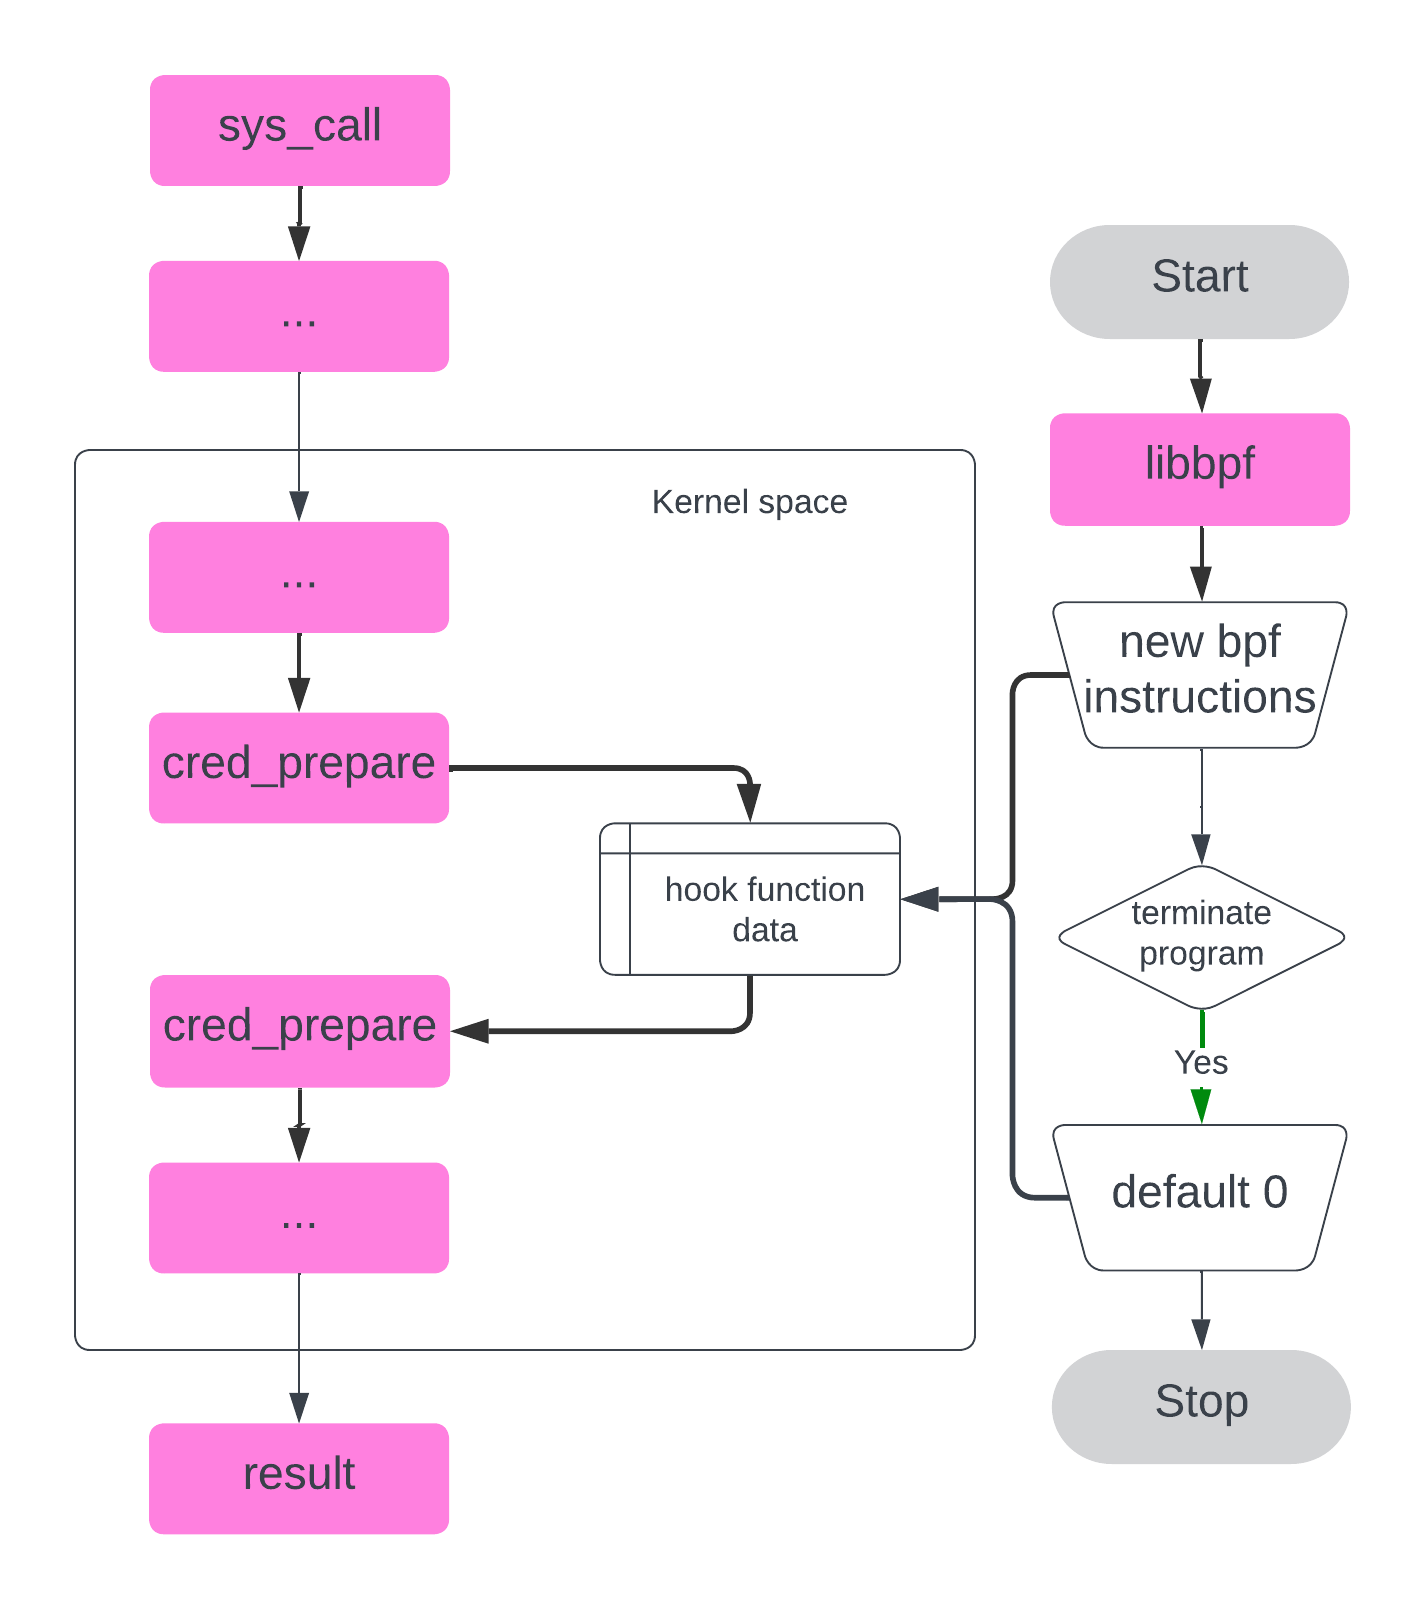
\includegraphics[width=\linewidth]{scheme.png}

\begin{flushleft}
	\ \\
	
	\ \\
	
	На данной схеме троеточием (...) обозначается незначительный процесс. Схема придерживается стандарта ГОСТ 19.701-90.
\end{flushleft}